\documentclass[aspectratio=169]{beamer}

\mode<presentation>
{
  \usetheme{default}
  \usecolortheme{default}
  \usefonttheme{default}
  \setbeamertemplate{navigation symbols}{}
  \setbeamertemplate{caption}[numbered]
  \setbeamertemplate{footline}[frame number]  % or "page number"
  \setbeamercolor{frametitle}{fg=white}
  \setbeamercolor{footline}{fg=black}
} 

\usepackage[english]{babel}
\usepackage[utf8x]{inputenc}
\usepackage{tikz}
\usepackage{courier}
\usepackage{array}
\usepackage{bold-extra}
\usepackage{minted}
\usepackage[thicklines]{cancel}

\xdefinecolor{dianablue}{rgb}{0.18,0.24,0.31}
\xdefinecolor{darkblue}{rgb}{0.1,0.1,0.7}
\xdefinecolor{darkgreen}{rgb}{0,0.5,0}
\xdefinecolor{darkgrey}{rgb}{0.35,0.35,0.35}
\xdefinecolor{darkorange}{rgb}{0.8,0.5,0}
\xdefinecolor{darkred}{rgb}{0.7,0,0}
\definecolor{darkgreen}{rgb}{0,0.6,0}
\definecolor{mauve}{rgb}{0.58,0,0.82}

\title[2017-12-13-ieee-bigdata]{Fast Access to Columnar, Hierarchical Data \\ via Code Transformation}
\author{Jim Pivarski$^1$, Peter Elmer$^1$, Brian Bockelman$^2$, and Zhe Zhang$^2$}
\institute{$^1$Princeton University, $^2$University of Nebraska at Lincoln -- DIANA-HEP}
\date{December 13, 2017}

\begin{document}

\logo{\pgfputat{\pgfxy(0.11, 7.4)}{\pgfbox[right,base]{\tikz{\filldraw[fill=dianablue, draw=none] (0 cm, 0 cm) rectangle (50 cm, 1 cm);}\mbox{\hspace{-9 cm}
\includegraphics[height=1 cm]{princeton-logo-long.png}
\includegraphics[height=1 cm]{nebraska-logo-long.png}
\includegraphics[height=1 cm]{diana-hep-logo-long.png}}}}}

\begin{frame}
  \titlepage
\end{frame}

\logo{\pgfputat{\pgfxy(0.11, 7.4)}{\pgfbox[right,base]{\tikz{\filldraw[fill=dianablue, draw=none] (0 cm, 0 cm) rectangle (50 cm, 1 cm);}\mbox{\hspace{-8 cm}
\includegraphics[height=1 cm]{princeton-logo.png}
\includegraphics[height=1 cm]{nebraska-logo.png}
\includegraphics[height=1 cm]{diana-hep-logo.png}}}}}

% Uncomment these lines for an automatically generated outline.
%\begin{frame}{Outline}
%  \tableofcontents
%\end{frame}

% START START START START START START START START START START START START START

\begin{frame}{My sliding definition of ``big data''}
\vspace{0.5 cm}
\begin{center}
\Large {\bf Big data (n.):} Techniques for handling datasets that are too big for a single computer.

\vspace{1 cm}
\uncover<2->{\textcolor{darkblue}{This is a moving target: different sizes in different decades.}}
\end{center}
\end{frame}

\begin{frame}{}

\begin{columns}
\column{1.15\linewidth}
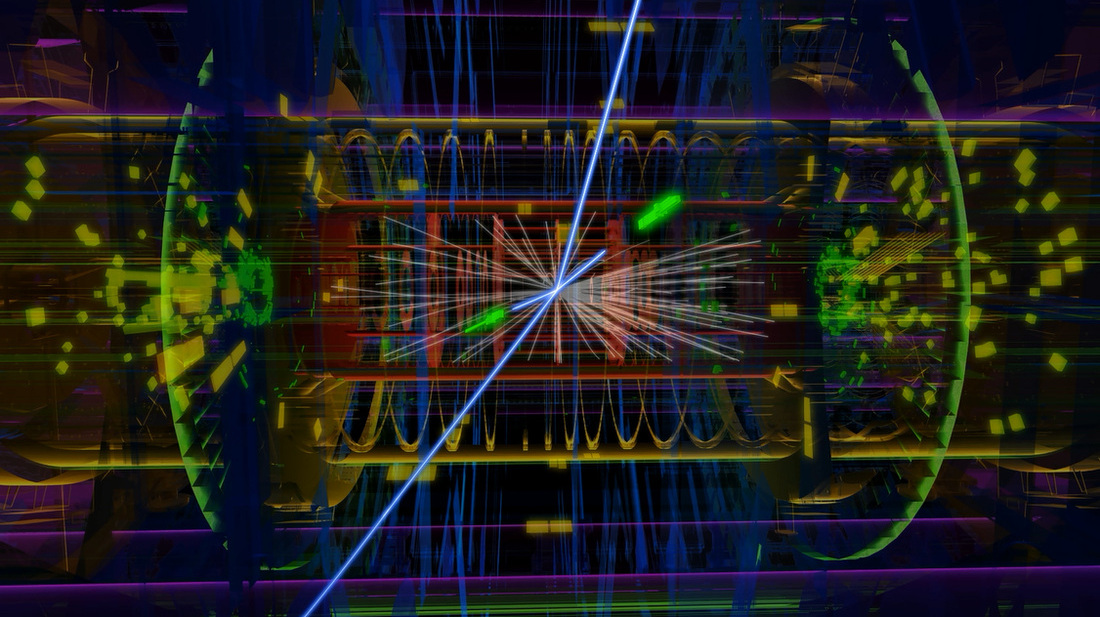
\includegraphics[width=\linewidth]{complex-atlas-collision-art.jpg}
\end{columns}

\vspace{-8.2 cm}
\uncover<1->{\textcolor{white}{\huge\bf In that sense, high-energy physicists have always dealt with big data.}}
\vspace{8.2 cm}
\end{frame}

\begin{frame}{High-energy physicists have always dealt with big data}
\vspace{0.5 cm}
\only<1>{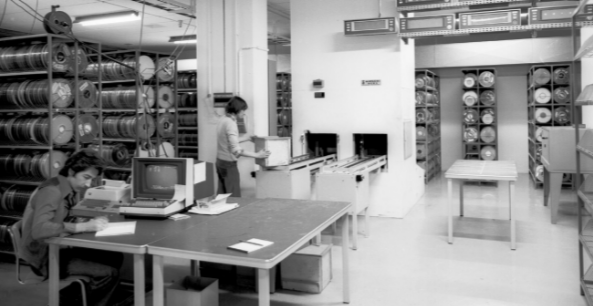
\includegraphics[width=\linewidth]{tapes1.png}}
\only<2>{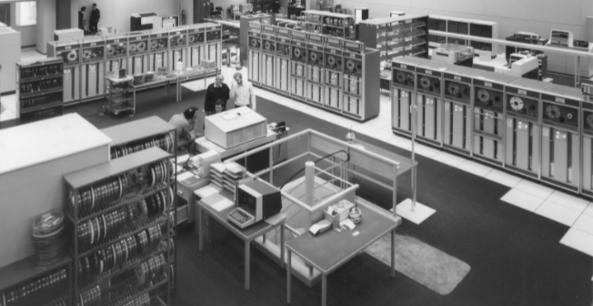
\includegraphics[width=\linewidth]{tapes2.png}}
\only<3>{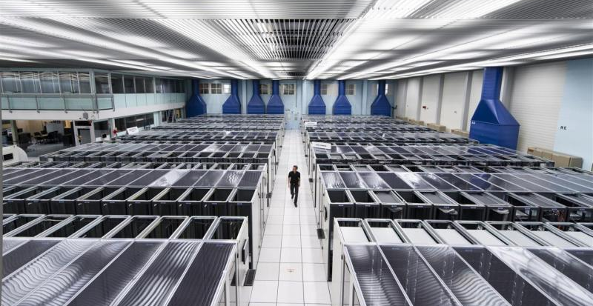
\includegraphics[width=\linewidth]{cerncomputing.png}}
\end{frame}

\begin{frame}{But we're certainly not the leaders in big data anymore}
\vspace{0.35 cm}
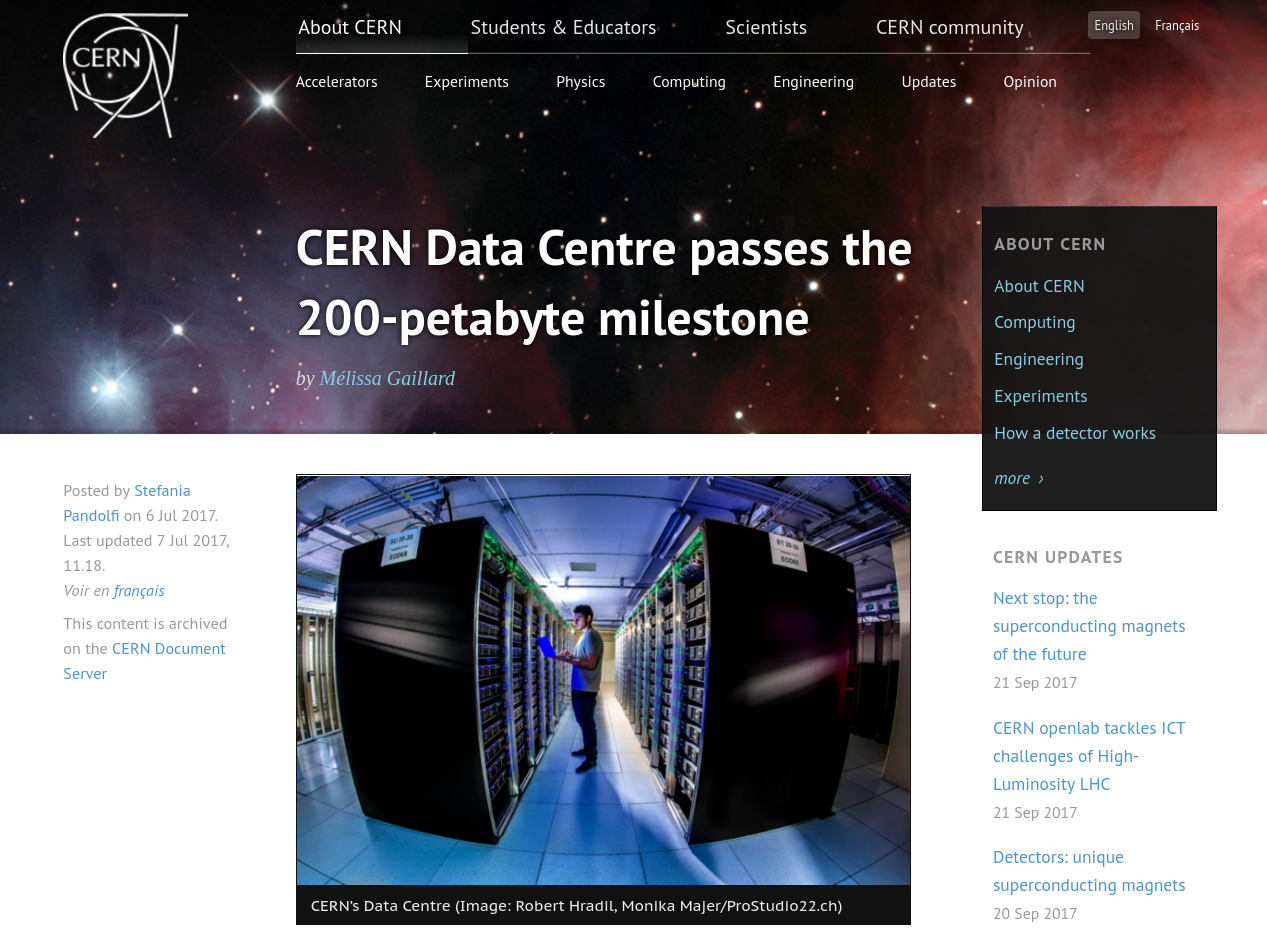
\includegraphics[width=0.73\linewidth]{cern-200pb.png}

\vspace{-4.8 cm}
\uncover<2->{\mbox{ } \hfill 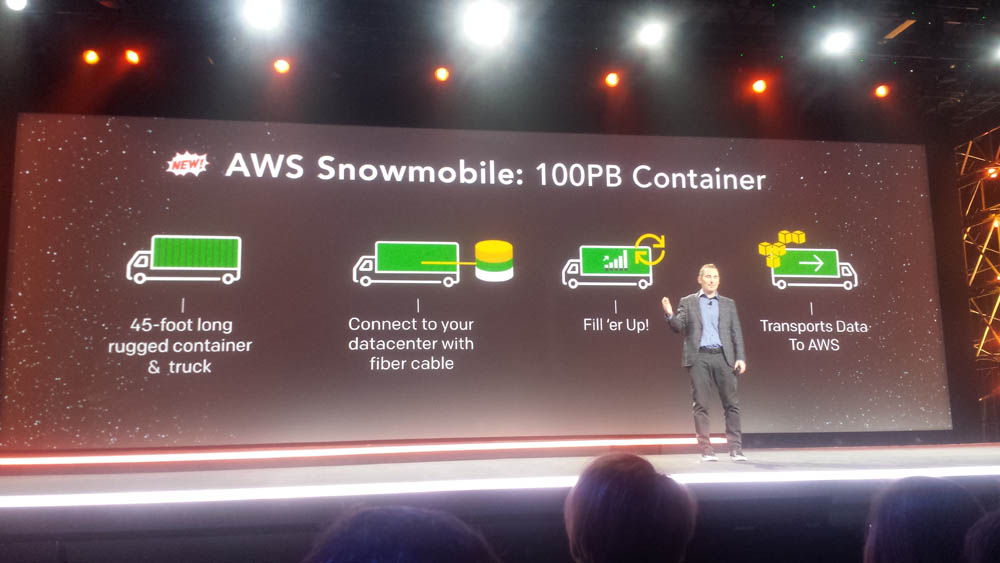
\includegraphics[width=0.7\linewidth]{aws-snowmobile.jpg}\hspace{-1 cm}}
\end{frame}

\begin{frame}{Data structure management in high-energy physics}
\vspace{0.25 cm}
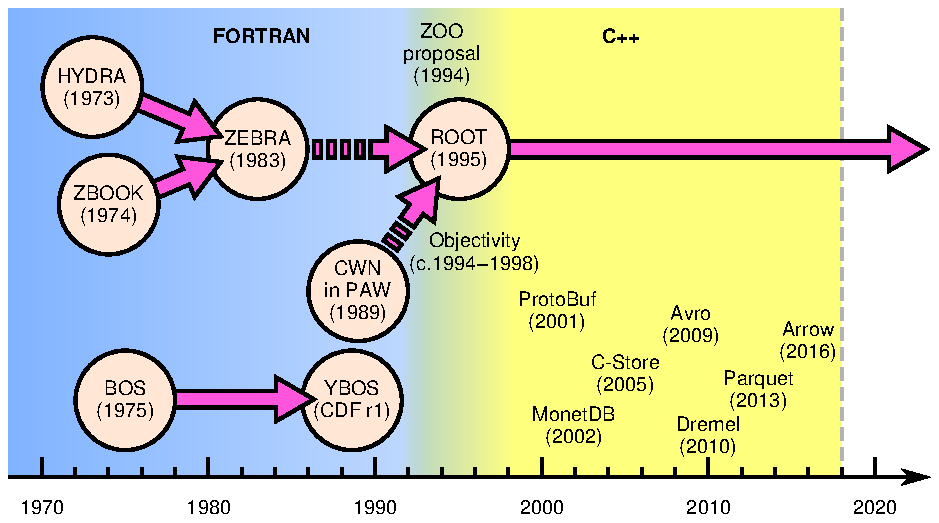
\includegraphics[width=\linewidth]{history.pdf}
\end{frame}

\begin{frame}[fragile]{High-energy physics data are arbitrary length lists}
\vspace{0.25 cm}
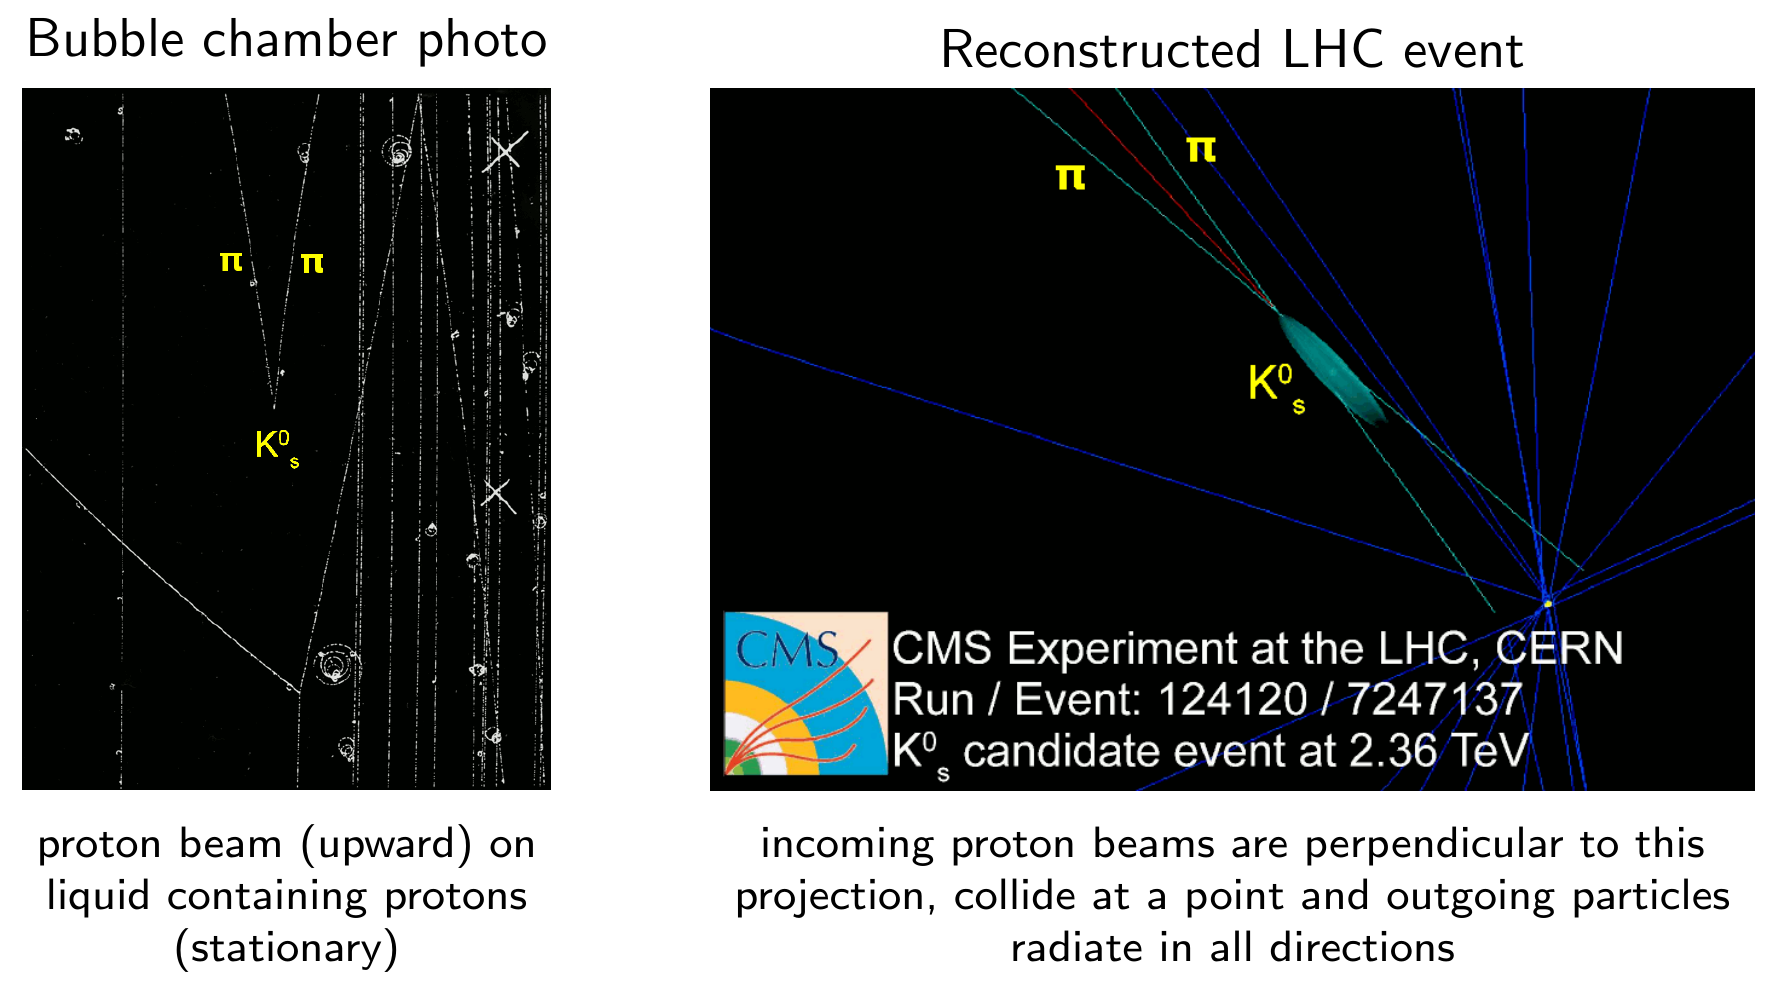
\includegraphics[width=\linewidth]{kshort.png}

\vspace{-7 cm}
\begin{uncoverenv}<2->
\begin{center}
\fcolorbox{black}{white}{\begin{minipage}{0.85\linewidth}
\begin{center}
\vspace{0.5 cm}
\begin{minipage}{0.85\linewidth}
Data are shaped like

\vspace{0.5 cm}
\only<2>{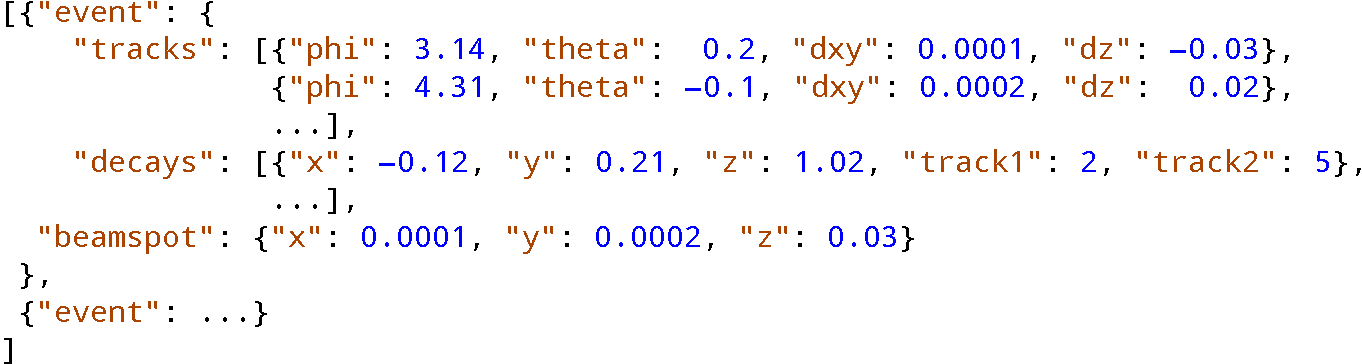
\includegraphics[width=\linewidth]{data-as-json-1.pdf}}
\only<3>{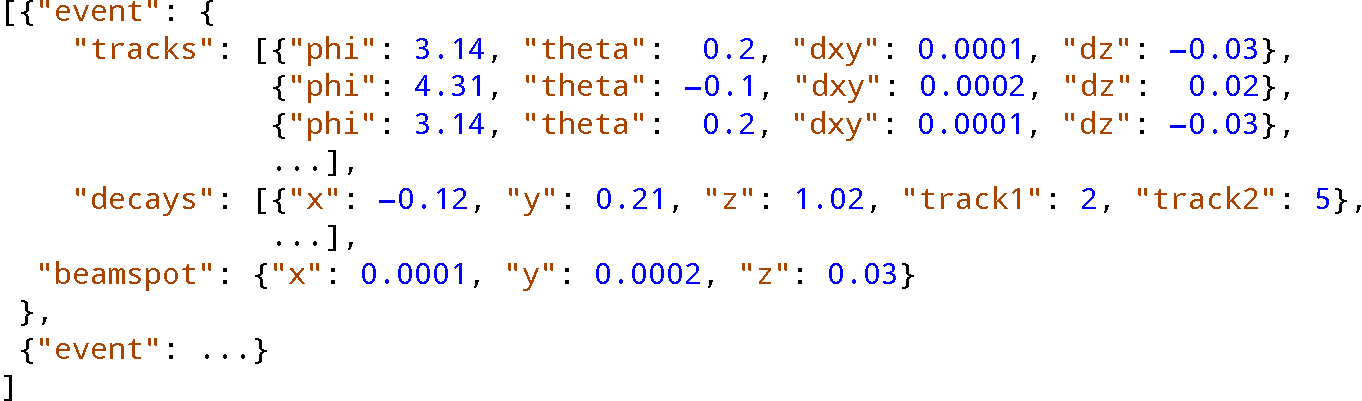
\includegraphics[width=\linewidth]{data-as-json-2.pdf}}
\only<4>{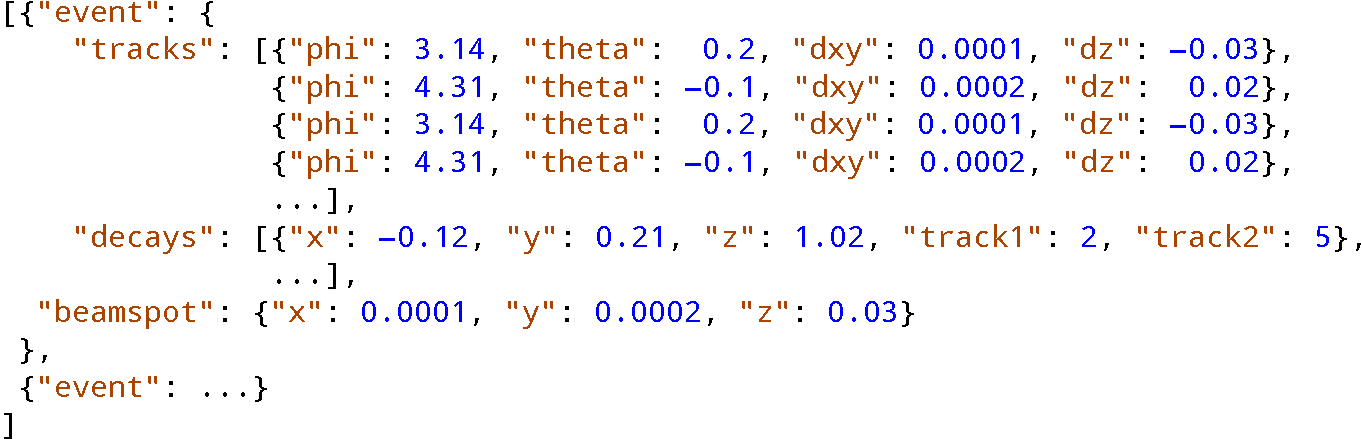
\includegraphics[width=\linewidth]{data-as-json-3.pdf}}

\only<3-4>{\vspace{0.5 cm}}
rather than a rectangular table with a fixed number of columns.
\end{minipage}
\vspace{0.5 cm}
\end{center}
\end{minipage}}
\end{center}
\end{uncoverenv}
\vspace{7 cm}
\end{frame}


\end{document}
